\documentclass[UTF8,a4paper,11pt]{ctexart}

\usepackage[a4paper,margin=2.5cm]{geometry}
\usepackage{graphicx}
\usepackage{subcaption}
\usepackage{mwe}
\usepackage{tikz}
\usepackage{amsmath,amssymb,amsthm}
\usepackage{siunitx}
\usepackage{booktabs}
\usepackage{array}
\usepackage{enumitem}
\usepackage{listings}
\usepackage{hyperref}
\usepackage{cleveref}
\usepackage{fancyhdr}
\usepackage{datetime2}
\usepackage{xcolor}
\usepackage{csquotes}

\hypersetup{
  colorlinks=true,
  linkcolor=blue,
  citecolor=teal,
  urlcolor=purple,
  pdftitle={LaTeX 快速入门与进阶实战},
  pdfauthor={Your Name}
}

\lstdefinestyle{codestyle}{
  basicstyle=\ttfamily\small,
  keywordstyle=\color{blue},
  commentstyle=\color{gray},
  stringstyle=\color{magenta},
  showstringspaces=false,
  frame=single,
  numbers=left,
  numberstyle=\tiny,
  breaklines=true,
  tabsize=2,
  captionpos=b
}
\lstset{style=codestyle}

\newtheorem{theorem}{定理}[section]
\newcommand{\code}[1]{\texttt{#1}}

\pagestyle{fancy}
\fancyhf{}
\fancyhead[L]{LaTeX 实战手册}
\fancyhead[R]{\leftmark}
\fancyfoot[C]{\thepage}
\setlength{\headheight}{15pt}

\title{LaTeX 快速入门与进阶实战手册\\
  \large 从基本语法到自动发布完整指南}
\author{示例作者}
\date{\DTMtoday}

\begin{document}

\maketitle
\tableofcontents
\clearpage

\section{为什么选择 \LaTeX}
与所见即所得编辑器不同,\LaTeX{} 提供可版本管理的纯文本工作流,便于多人协作、严谨排版与自动化构建。本手册以实战为导向,帮助你在本仓库中快速掌握从基础到高级的主流技巧。若你已安装 MacTeX,那么你已经拥有全部所需的编译工具链。

\section{文档基本结构}\label{sec:structure}
典型的 \LaTeX{} 文件分为导言区(在 \verb|\begin{document}| 之前)与正文区(在 \verb|\begin{document}| 与 \verb|\end{document}| 之间)。

\subsection{导言区要素}
\begin{itemize}[leftmargin=2em]
  \item \textbf{文档类:}决定整体版式,例如 \verb|ctexart| 适合中文文章;\verb|beamer| 用于幻灯片;\verb|report| 用于长文档。
  \item \textbf{宏包加载:}使用 \verb|\usepackage| 引入功能扩展;宏包通常带有可选参数,例如 \verb|\usepackage[margin=2.5cm]{geometry}|。
  \item \textbf{自定义命令:}通过 \verb|\newcommand| 封装常用结构,提高文档可维护性。
\end{itemize}

\subsection{正文区组件}
正文区由标题页、章节结构、图表、公式等构成。参见本文件末尾附录 \ref{sec:cheatsheet} 获取常用指令速查。

\section{文字与段落排版}
基础段落直接输入文本即可,空行代表新的段落。常用强调方式如下:
\begin{itemize}[leftmargin=2em]
  \item \verb|\textbf{粗体}|,\verb|\textit{斜体}| 与 \verb|\underline{下划线}|。
  \item \verb|\emph{重点}| 会根据上下文在粗体或斜体之间自动切换。
  \item 等宽字体使用 \verb|\code{控制命令}|。
\end{itemize}

\subsection{列表}
\begin{minipage}{0.48\textwidth}
\begin{verbatim}
\begin{itemize}
  \item 无序列表
\end{itemize}
\end{verbatim}
\end{minipage}
\hfill
\begin{minipage}{0.48\textwidth}
\begin{itemize}
  \item 支持嵌套
  \item 可用 enumitem 调整缩进
\end{itemize}
\end{minipage}

有序列表与描述列表分别使用 \verb|enumerate| 与 \verb|description| 环境,并可借助 \verb|enumitem| 宏包调整标签样式。

\section{数学公式与定理环境}\label{sec:math}
数学是 \LaTeX{} 的强项。内联公式使用 \verb|$...$| 包裹,例如 $E = mc^2$;独立行公式使用 \verb|\[ ... \]| 或 \verb|\begin{equation} ... \end{equation}|。

\subsection{常见环境}
\begin{align}
\int_{0}^{\infty} e^{-x^2} \, \mathrm{d}x &= \frac{\sqrt{\pi}}{2}, \label{eq:gauss}\\
\mathbf{A}\mathbf{x} &= \mathbf{b} \tag{\text{线性方程组}}
\end{align}
多行公式可使用 \verb|align|、\verb|cases|、\verb|split| 等环境。

\begin{theorem}[勾股定理]\label{thm:pythagorean}
在直角三角形中,斜边长度平方等于两条直角边长度平方之和:若直角边为 $a, b$,斜边为 $c$,则有 $a^2 + b^2 = c^2$。
\end{theorem}

引用公式 \cref{eq:gauss} 或定理 \cref{thm:pythagorean} 时,\texttt{cleveref} 会自动选择合适的标签。

\section{图像、表格与浮动体}
\LaTeX{} 使用浮动体管理图表位置。图(figure)和表(table)均可带标题与标签。

\subsection{插入图片}
\cref{fig:image-demo} 演示了如何插入图片与并排子图。

\begin{figure}[htbp]
  \centering
  \begin{subfigure}[b]{0.45\textwidth}
    \centering
    \includegraphics[width=\linewidth]{example-image}
    \caption{示例图像}
  \end{subfigure}
  \hfill
  \begin{subfigure}[b]{0.45\textwidth}
    \centering
    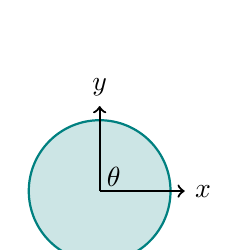
\begin{tikzpicture}[scale=0.9]
      \filldraw[fill=teal!20, draw=teal, thick] (0,0) circle (1);
      \draw[->, thick] (0,0) -- (1.2,0) node[right] {$x$};
      \draw[->, thick] (0,0) -- (0,1.2) node[above] {$y$};
      \node at (0.2,0.2) {$\theta$};
    \end{tikzpicture}
    \caption{TikZ 绘图}
  \end{subfigure}
  \caption{图像与 TikZ 并排示例}\label{fig:image-demo}
\end{figure}

\subsection{表格}
使用 \verb|tabular| 环境创建表格,\verb|booktabs| 宏包提供更专业的横线。
\begin{table}[htbp]
  \centering
  \caption{实验结果示例}\label{tab:results}
  \begin{tabular}{@{}lS[round-mode=places,round-precision=2]S[table-format=2.2]@{}}
    \toprule
    指标 & {基线模型} & {改进模型} \\
    \midrule
    准确率 (\%) & 82.34 & 91.57 \\
    F1 分数     & 0.78  & 0.88  \\
    耗时 (s)    & 125   & 98    \\
    \bottomrule
  \end{tabular}
\end{table}
引用 \cref{tab:results} 时,\texttt{cleveref} 会自动生成“表~\ref{tab:results}”样式。

\section{交叉引用、脚注与文献}\label{sec:references}
交叉引用的基本步骤:
\begin{enumerate}[leftmargin=2em]
  \item 在目标对象后添加 \verb|\label{key}|。
  \item 在需要引用的位置使用 \verb|\ref{key}| 或 \verb|\cref{key}|。
  \item 编译两次(或使用 \verb|latexmk|)以更新引用。
\end{enumerate}

脚注示例:这是一个内联脚注\footnote{脚注适合补充说明,不宜写过长。}。

文献管理推荐使用 Bib\TeX{}:在 \code{refs.bib} 中维护条目,然后通过 \verb|\cite{key}| 引用,例如 \cite{lamport1994latex}。完整列表将在文末打印。

\section{代码与算法排版}\label{sec:code}
\texttt{listings} 宏包可高亮代码。若你希望使用 Pygments 渲染,可换用 \texttt{minted} 宏包,并在编译时加入 \code{-shell-escape}。

\begin{lstlisting}[language=Python,caption={使用 SymPy 验证勾股恒等式}]
from sympy import symbols, Eq, simplify

a, b = symbols("a b", positive=True)
c_square = a**2 + b**2
hypotenuse = simplify(c_square)
assert Eq(hypotenuse, a**2 + b**2)
\end{lstlisting}

算法排版可借助 \texttt{algorithm2e}、\texttt{algorithmic} 等宏包(视需求引入)。

\section{页面样式与宏命令}
宏包 \texttt{fancyhdr} 可以自定义页眉页脚,本文件的页眉即通过 \verb|\fancyhead| 设置。可使用 \verb|\newcommand| 封装常用格式,例如:
\begin{verbatim}
\newcommand{\R}{\mathbb{R}}
\end{verbatim}

配合 \verb|geometry| 调整边距、\verb|setstretch| (来自 \texttt{setspace} 宏包) 调整行距,可快速获得符合期刊/学校要求的版式。

\section{自动化构建与发布流程}\label{sec:automation}
在现代工作流中,建议使用 \verb|latexmk| 管理编译流程,配合 Git 版本控制实现“一键发布”。

\subsection{命令行自动化}
\begin{enumerate}[leftmargin=2em]
  \item 执行 \verb|make pdf| 调用 \code{latexmk} 持续编译并生成 \code{build/main.pdf}。
  \item 执行 \verb|make clean| 清理中间文件。
  \item 运行 \verb|./publish.sh "更新说明"| 自动编译并将 PDF 与源码提交到当前 Git 远端(需提前配置远端分支)。
\end{enumerate}

\subsection{LaTeX Workshop 集成}
在 VS Code 中:
\begin{enumerate}[leftmargin=2em]
  \item 打开命令面板,选择 “\code{LaTeX Workshop: Create LaTeX Project}” 或直接打开本仓库。
  \item 确保设置 \code{"latex-workshop.latex.tools"} 包含 \code{latexmk},并在 \code{"latex-workshop.latex.recipes"} 中选择 \code{latexmk (xelatex)}。
  \item 使用 “\code{Build LaTeX project}” 触发本地编译;\LaTeX{} Workshop 会根据 \code{latexmkrc} 自动调用 XeLaTeX 并输出 PDF。
  \item 可在设置中开启 \code{"latex-workshop.view.pdf.viewer": "tab"} 实现编译后自动预览。
\end{enumerate}

\subsection{Git 上传提醒}
推荐的 Git 提交流程:
\begin{enumerate}[leftmargin=2em]
  \item \verb|git status| 查看改动。
  \item \verb|git add main.tex refs.bib Makefile latexmkrc publish.sh|
  \item \verb|git commit -m "docs: 更新 LaTeX 教程"| 
  \item \verb|git push origin <your-branch>|
\end{enumerate}
如使用 \code{publish.sh},脚本会自动执行上述步骤并附加时间戳。

\section{扩展资源与进阶推荐}
\begin{itemize}[leftmargin=2em]
  \item 官方 \href{https://www.latex-project.org/help/documentation/}{\LaTeX{} Project 文档}。
  \item \href{https://ctan.org/}{CTAN} 宏包索引,可搜索任意宏包说明。
  \item \href{https://tex.stackexchange.com/}{TeX StackExchange} 是解决疑难问题的最佳社区。
  \item \LaTeX{} 参考书籍如 \cite{mittelbach2004latex} 提供系统化学习路径。
\end{itemize}

\appendix
\section{常用指令速查}\label{sec:cheatsheet}
\begin{itemize}[leftmargin=2em]
  \item \textbf{段落与章节:} \verb|\section|、\verb|\subsection|、\verb|\paragraph|。
  \item \textbf{数学:} \verb|\frac|、\verb|\sqrt|、\verb|\sum|、\verb|\int|、\verb|\mathbf|、\verb|\mathbb|。
  \item \textbf{引用:} \verb|\label| + \verb|\ref|;\verb|\cite| 用于文献。
  \item \textbf{图表:} \verb|\includegraphics| 与 \verb|tabular|。
  \item \textbf{布局:} \verb|\begin{minipage}{宽度}|、\verb|\vspace|、\verb|\hfill|。
  \item \textbf{调试:} \verb|\usepackage{showframe}| 查看页面边界;\verb|\listfiles| 输出依赖宏包版本。
\end{itemize}

\bibliographystyle{ieeetr}
\bibliography{refs}

\end{document}
